% Estas slides tienen que abrirse con el programa pdfpc que soporta videos embebidos
% el comando es: pdfpc -g slides.pdf
% para los videos se requiere ubuntu-restricted-extras
% para la bibliografía se requiere biber y configurar texstudio

%\documentclass[compress,handout]{beamer}
\documentclass[aspectratio=169,compress]{beamer}

% add beamer preamble
% In this preamble should go only package and settings related with beamer

% Theme customization
\setbeamertemplate{itemize item}[rectangle] % configure itemize
\setbeamertemplate{itemize subitem}[circle] % configure itemize
\setbeamertemplate{itemize subsubitem}[triangle] % configure itemize
\setbeamertemplate{navigation symbols}{} % remover simbolos de navegacion de las slides
\usefonttheme[onlymath]{serif} % simbolos matematicos en serif (Como es en latex original)
\setbeamersize{text margin left=3mm,text margin right=3mm} 

\setbeamertemplate{blocks}[rounded] % blocks corners rounded
\setbeamercolor{block body}{bg=blue!12,fg=black} % color of blocks
\setbeamertemplate{caption}{\raggedright\insertcaption\par} % elimina la palabra "Figura" del caption

\usepackage[overridenote]{pdfpc} % requires to download manually pdfpc.sty package from https://www.ctan.org/pkg/pdfpc
% para instalar el pdfpc.sty seguir las instrucciones en https://micropore.wordpress.com/2009/11/28/texhash/

%\setbeameroption{show notes on second screen=right} % visualize slides with notes using beamerpresenter slides.pdf

% HOW TO SHOW ADDITIONAL SLIDES%
\newif\ifadditional % conditional to show additional slides
%\additionaltrue   % uncomment to show additional slides
\additionalfalse % uncomment to show without additional slides

% Reference cite without footnote mark
\newrobustcmd*{\footfullcitenomark}{%
    \AtNextCite{%
        \let\thefootnote\relax
        \let\mkbibfootnote\mkbibfootnotetext}%
    \footfullcite}


% add latex preamble
% para la bibliografía se requiere biber y configurar texstudio

% Latex packages
\usepackage[utf8]{inputenc}
\usepackage[T1]{fontenc} % para copiar acentos en español del pdf y permite acentos en las notas
\usepackage[english]{babel}
\usepackage[per-mode = symbol]{siunitx} % para manejar las unidades
\usepackage{multimedia} % to add videos with \movie command
\usepackage{multirow}
\usepackage{graphicx}
\usepackage{xcolor}
\usepackage{amsmath} % bmatrix
\usepackage[makeroom]{cancel} % \cancel to cancel terms in math equations
\renewcommand{\CancelColor}{\color{red}} % set red color for \cancel command
\usepackage[caption=false]{subfig} % caption = false elimina la palabra "Figura" del caption
\usepackage{import} % para el comando import (se usa para pdf_tex)
\captionsetup[subfigure]{labelformat=empty} % remover el indice del caption de la subfigura
\usepackage{booktabs} % \toprule \midrule \bottomrule
\usepackage[backend=biber]{biblatex} % set biber to format references. Must configure Biber in Texstudio
\usepackage{csquotes} % to remove warning triggered by biblatex and babel
\usepackage{algorithm} % to put captions to the algorithmics environmets
\usepackage{algpseudocode} % to write algorithm
\usepackage{tikz} % to use tikz
\usepackage[export]{adjustbox} %valign in subfloat
\usepackage{colortbl} % to paint cells in a table

% Color commands for annotations
\newcommand\TODO[1]{\textbf{\textcolor{red}{#1}}} %  TODO notes

% Graphic paths
\graphicspath{{./images/}}

% listings configuration for C code
\usepackage{listings} % code
\definecolor{commentgreen}{RGB}{2,112,10}
\definecolor{eminence}{RGB}{108,48,130}
\definecolor{weborange}{RGB}{255,165,0}
\definecolor{frenchplum}{RGB}{129,20,83}

\lstset{ % spanish characters for listings package
	inputencoding=latin1,
    columns=fullflexible,
	breaklines=true,
	tabsize=2,
	showstringspaces=false,
	basicstyle=\ttfamily,
	backgroundcolor=\color{lightgray}, % Choose background color
	literate={á}{{\'a}}1
	{ã}{{\~a}}1
	{é}{{\'e}}1
	{ó}{{\'o}}1
	{í}{{\'i}}1
	{ñ}{{\~n}}1
	{¡}{{!`}}1
	{¿}{{?`}}1
	{ú}{{\'u}}1
	{Í}{{\'I}}1
	{Ó}{{\'O}}1
    {-}{-}1
}

\lstdefinestyle{cpp}{ % spanish characters for listings package
    language=C++,
   	commentstyle=\color{commentgreen},
    keywordstyle=\color{eminence},
    stringstyle=\color{red},
    emph={int,char,double,float,unsigned,void,bool},
    emphstyle={\color{blue}}
}

\lstdefinestyle{bash}{ % spanish characters for listings package
	language=Bash
}

\lstdefinestyle{xml}{
	language=XML,
	morekeywords={encoding,xs:schema,xs:element,xs:complexType,xs:sequence,xs:attribute}
}

\lstdefinestyle{cmake}{
	language=make, % there is no cmake support in listings
}

\lstdefinestyle{python}{
    language=python,
}


%%%%% PARA QUE EN LAS TABLAS SE PUEDA PONER UN SALTO DE LINEA DENTRO DE UNA CELDA
\newcommand{\specialcell}[2][c]{%
    \begin{tiny}
        \begin{tabular}[#1]{@{}c@{}}#2\end{tabular}  
    \end{tiny}
}
%%%%%%%%%%%%%%%%%%%%%%%%%%%%%%%%%%%%%%%%%%%%%%%%%%%%%%%%%%%%%%%%%%%%%%%%

%%%%% PARA QUE LAS TABLAS TENGAN TODAS LAS COLUMNAS CENTRADAS Y DE IGUAL TAMAÑO
\usepackage{tabularx}
\renewcommand{\tabularxcolumn}[1]{>{\centering\arraybackslash}m{#1}}
%%%%%%%%%%%%%%%%%%%%%%%%%%%%%%%%%%%%%%%%%%%%%%%%%%%%%%%%%%%%%%%%%%%%%%%%



% add math preamble
\usepackage{amsmath}
\usepackage{amssymb}
\usepackage{amsopn}
\usepackage{mathtools}

% set matrix maximum length
\setcounter{MaxMatrixCols}{20}

% math
\renewcommand{\vec}[1]{\boldsymbol{\mathbf{#1}}}
\newcommand{\norm}[1]{\lVert#1\rVert}

% Declare arg max and arg min functionss
\DeclareMathOperator*{\argmax}{arg\,max}
\DeclareMathOperator*{\argmin}{arg\,min}

% Declare atan2 
\DeclareMathOperator{\atantwo}{atan2}

% Homogeneous decoration function
\newcommand{\homo}[1]{\dot{#1}}


% Declare projection as math function
\DeclareMathOperator{\proj}{proj}
\newcommand{\fromCoord}[2]{{#1}_\mathrm{#2}}
\newcommand{\toCoord}[2]{\prescript{\mathrm{#2}}{}{#1}}
\newcommand{\worldCoordSystem}{\mathrm{W}}
\newcommand{\bodyCoordSystem}{\mathrm{B}}
\newcommand{\cameraCoordSystem}{\mathrm{C}}
\newcommand{\origin}{\vec{o}}
\newcommand{\point}{\vec{p}}
\newcommand{\worldPoint}{\toCoord{\point}{\worldCoordSystem}}
\newcommand{\imagePoint}{\vec{u}}
\newcommand{\cameraPoint}{\toCoord{\point}{\cameraCoordSystem}}
\newcommand{\homoWorldPoint}{\toCoord{\homo{\point}}{\worldCoordSystem}}
\newcommand{\homoImagePoint}{\homo{\imagePoint}}
\newcommand{\homoCameraPoint}{\toCoord{\homo{\point}}{\cameraCoordSystem}}
\newcommand{\measurement}{\vec{z}}
\newcommand{\prediction}{\hat{\vec{z}}}
\newcommand{\seMatrix}{\vec{\xi}}
\newcommand{\transform}[2]{\toCoord{\fromCoord{\seMatrix}{#2}}{#1}}
\newcommand{\pointCoord}[1]{\toCoord{\point}{#1}}
\newcommand{\rotation}{\vec{R}}
\newcommand{\rotationCoord}[2]{\toCoord{\fromCoord{\rotation}{#2}}{#1}}
\newcommand{\translation}{\vec{t}}
\newcommand{\translationCoord}[2]{\toCoord{\fromCoord{\translation}{#2}}{#1}}
\newcommand{\intrinsicMatrix}{\vec{K}}
\newcommand{\principalPoint}{\vec{c}}
\newcommand{\reprojectionError}{u}
\newcommand{\projectionMatrix}{\vec{P}}
\newcommand{\cameraCenter}{\vec{o}}
\newcommand{\worldCameraCenter}{\toCoord{\cameraCenter}{\worldCoordSystem}}
\newcommand{\essentialMatrix}{\vec{E}}
\newcommand{\fundamentalMatrix}{\vec{F}}
\newcommand{\inverse}[1]{{#1}^{-1}}
\newcommand{\epipole}{\vec{e}}

% Localization (State Estimation)
\newcommand{\state}{x}
\newcommand{\observation}{z}
\newcommand{\controlCommand}{u}
\newcommand{\covariance}{\Sigma}
\newcommand{\motionModelNoise}{\epsilon}
\newcommand{\measurementModelNoise}{\delta}
\newcommand{\motionModelFunction}[1]{g\left( #1 \right)}
\newcommand{\observationModelFunction}[1]{h\left( #1 \right)}
\newcommand{\motionParametersCovariance}{R}
\newcommand{\observationModelCovariance}{Q}
\newcommand{\motionModelJacobian}{G}
\newcommand{\observationModelJacobian}{H}
\newcommand{\kalmanGain}{K}
\newcommand{\normalDistribution}[2]{\mathcal{N}\left( {#1}, {#2} \right)}
\newcommand{\motionModelJacobianControl}{V}
\newcommand{\motionModelCovariance}{M}
\newcommand{\stateEvolutionMatrix}{A}

% Mapping slides
\newcommand{\map}{m}
\newcommand{\mapRandomVariable}{m}

% SLAM slides
\newcommand{\informationMatrix}{\vec{\Omega}}
\newcommand{\error}{\vec{e}}
\newcommand{\observationBold}{\vec{z}}
\newcommand{\stateBold}{\vec{x}}
\newcommand{\jacobian}{\vec{J}}
\newcommand{\linearSystemb}{\vec{b}}
\newcommand{\linearSystemH}{\vec{H}}


% Motion Planning slides
\newcommand{\workSpace}{\mathcal{W}}
\newcommand{\obstaclesSet}{\mathcal{O}}
\newcommand{\robotInConfiguration}{\mathcal{A}}
\newcommand{\robotConfiguration}{q}
\newcommand{\configurationSpace}{\mathcal{C}}
\newcommand{\freeConfigurationSpace}{\configurationSpace_{free}}
\newcommand{\obstableConfigurationSpace}{\configurationSpace_{obs}}
\newcommand{\goalSet}{\configurationSpace_{goal}}
\newcommand{\startConfiguration}{\robotConfiguration_{I}}
\newcommand{\goalConfiguration}{\robotConfiguration_{G}}
\newcommand{\continuousPath}{\tau}
\newcommand{\motionLaw}{\gamma}
\newcommand{\robotActionSpace}{\mathcal{U}}


% Motion model
\newcommand{\position}{\vec{p}}
\newcommand{\orientation}{\vec{O}}
\newcommand{\orientationQuaternion}{\vec{q}}
\newcommand{\predictedPosition}{\hat{\vec{p}}}
\newcommand{\predictedOrientationQuaternion}{\hat{\vec{q}}}
\newcommand{\linearVelocity}{\vec{v}}
\newcommand{\angularVelocity}{\vec{\omega}}

\DeclareMathOperator{\slerpOp}{slerp}
\newcommand{\slerp}[1]{\slerpOp{\left( #1 \right)}}

% Map structure
\newcommand{\keyframesSet}{K}
\newcommand{\mapPointsSet}{P}
\newcommand{\observedMapPoints}{O}
\newcommand{\covisibilityKeyframes}{CK}
\newcommand{\localMap}{local\_map}

% Bundle Adjutment
\newcommand{\update}{\vec{\delta}}
\newcommand{\incremental}{\hat{\update}}


% Loop Closure names

% scaled operators and letters to fancy view
\newcommand{\sminus}{\scalebox{0.5}[1.0]{$-$}}
\newcommand{\splus}{\scalebox{0.6}[0.6]{$+$}}
\newcommand{\curr}{c}
\newcommand{\sind}[1]{\scalebox{0.6}[0.6]{$#1$}}
\newcommand{\ind}[1]{\scalebox{0.7}[0.7]{$#1$}}

\newcommand{\keyframe}{\vec{K}}
\newcommand{\bowVector}{\vec{v}}
\newcommand{\lcError}{\vec{\Omega}}
\newcommand{\relativeTransformation}{\seMatrix}
\DeclareMathOperator{\interpolate}{interpolate}

\newcommand{\relativeMotion}{\vec{\delta}}
\newcommand{\groundTruth}[1]{{#1}^{*}}

% definición del operador rot()
\DeclareMathOperator{\rotationOp}{rot}
\newcommand{\getRotation}[1]{\rotationOp{\left( #1 \right)}}

\DeclareMathOperator{\translationOp}{trans}
\newcommand{\getTranslation}[1]{\translationOp{\left( #1 \right)}}









% add bibliography resource
\renewcommand*{\bibfont}{\footnotesize} % change bibliograhy size
\bibliography{../../common/bibliography.bib}

\subtitle{SLAM: Simultaneous Localization and Mapping}
\title{Robótica Móvil}
\author{Taihú Pire}
\institute{Laboratorio de Robótica}
\titlegraphic{
\includegraphics[width=0.4\textwidth]{images/cifasis_logo.pdf}}
\date{}

\begin{document}
	
	% add title page
	\frame{\titlepage}
	
	\section{SLAM}
	\begin{frame}
    \frametitle{Analyze for these slides}
    
    \begin{itemize}
    \item EKF-SLAM
    \item Graph-SLAM / Factor Graph
    \item Loop-Closure
    \item Bundle Adjustment
    \end{itemize}
    
    \end{frame}
    
    \begin{frame}
    \frametitle{What is SLAM?}
    
    For a mobile robot to navigate autonomously, it must know its location and have a representation of the environment it is in. These problems are known as the Localization and Mapping problems. In the most general case, where neither the robot's location nor an a priori map of the environment is available, these problems are addressed simultaneously. This gives rise to the SLAM problem (\emph{Simultaneous Localization and Mapping}).
    \begin{block}{}
    SLAM is the problem of solving localization and mapping at the same time.
    \end{block}
    
    \end{frame}
    
    
    \begin{frame}
     \frametitle{SLAM example}
    
     \begin{figure}
     \subfloat[Reality]
     {
     \fbox{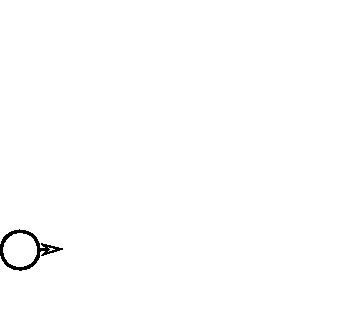
\includegraphics[width=0.44\textwidth]{slam_example_gt1.pdf}}
     }\hfill{}
     \subfloat[Robot SLAM system]
     {
     \fbox{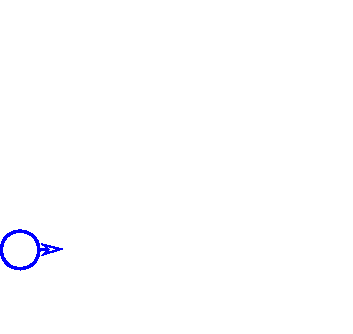
\includegraphics[width=0.44\textwidth]{slam_example_robot1.pdf}}
     }
     \end{figure}
    
    \end{frame}
    
    \begin{frame}
     \frametitle{SLAM example}

     \begin{figure}
     \subfloat[Reality]
     {
     \fbox{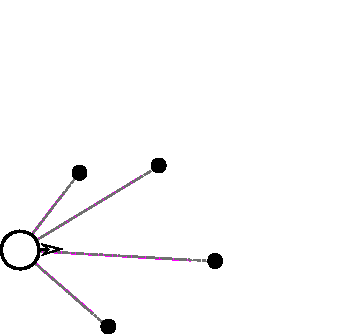
\includegraphics[width=0.44\textwidth]{slam_example_gt2.pdf}}
     }\hfill{}
     \subfloat[Robot SLAM system]
     {
     \fbox{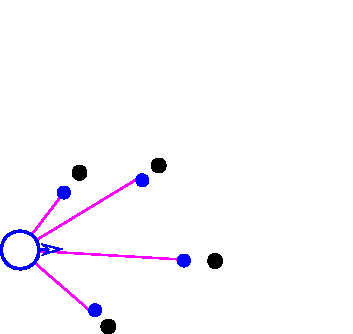
\includegraphics[width=0.44\textwidth]{slam_example_robot2.pdf}}
     }
     \end{figure}
    
    \end{frame}
    
    \begin{frame}
     \frametitle{SLAM example}
    
     \begin{figure}
     \subfloat[Reality]
     {
     \fbox{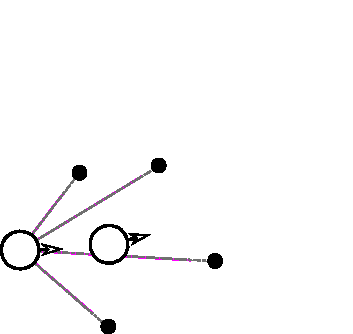
\includegraphics[width=0.44\textwidth]{slam_example_gt3.pdf}}
     }\hfill{}
     \subfloat[Robot SLAM system]
     {
     \fbox{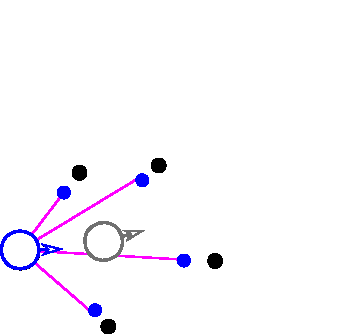
\includegraphics[width=0.44\textwidth]{slam_example_robot3.pdf}}
     }
     \end{figure}
    
    \end{frame}
    
    \begin{frame}
     \frametitle{SLAM example}
    
     \begin{figure}
     \subfloat[Reality]
     {
     \fbox{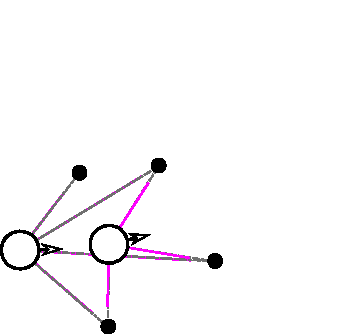
\includegraphics[width=0.44\textwidth]{slam_example_gt4.pdf}}
     }\hfill{}
     \subfloat[Robot SLAM system]
     {
     \fbox{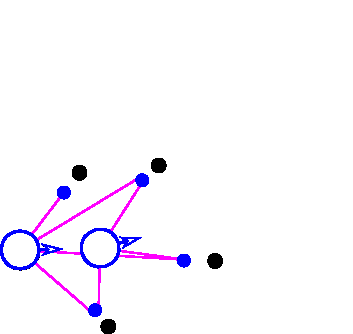
\includegraphics[width=0.44\textwidth]{slam_example_robot4.pdf}}
     }
     \end{figure}
    
    \end{frame}
    
    \begin{frame}
     \frametitle{SLAM example}
    
     \begin{figure}
     \subfloat[Reality]
     {
     \fbox{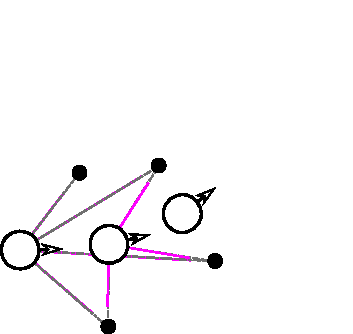
\includegraphics[width=0.44\textwidth]{slam_example_gt5.pdf}}
     }\hfill{}
     \subfloat[Robot SLAM system]
     {
     \fbox{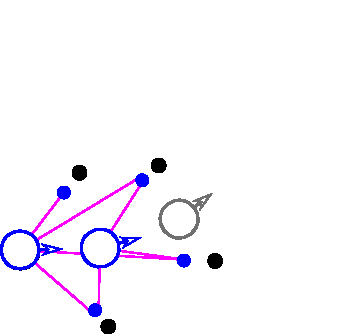
\includegraphics[width=0.44\textwidth]{slam_example_robot5.pdf}}
     }
     \end{figure}
    
    \end{frame}
    
    \begin{frame}
     \frametitle{SLAM example}
    
     \begin{figure}
     \subfloat[Reality]
     {
     \fbox{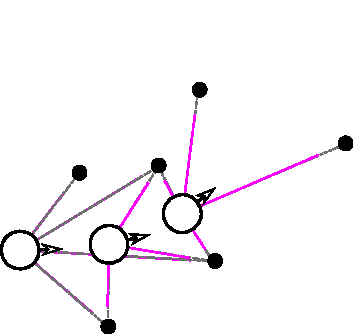
\includegraphics[width=0.44\textwidth]{slam_example_gt6.pdf}}
     }\hfill{}
     \subfloat[Robot SLAM system]
     {
     \fbox{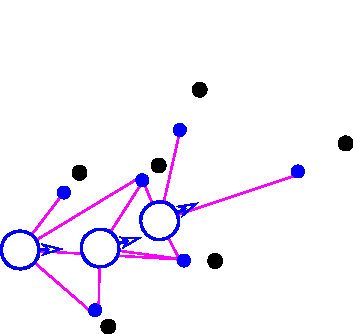
\includegraphics[width=0.44\textwidth]{slam_example_robot6.pdf}}
     }
     \end{figure}
    
    \end{frame}
    
    \begin{frame}
     \frametitle{SLAM example}
    
     \begin{figure}
     \subfloat[Reality]
     {
     \fbox{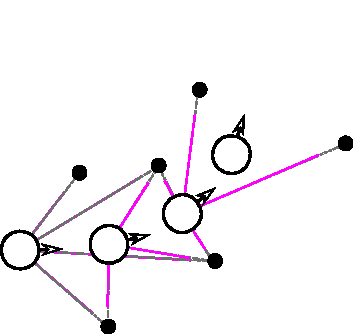
\includegraphics[width=0.44\textwidth]{slam_example_gt7.pdf}}
     }\hfill{}
     \subfloat[Robot SLAM system]
     {
     \fbox{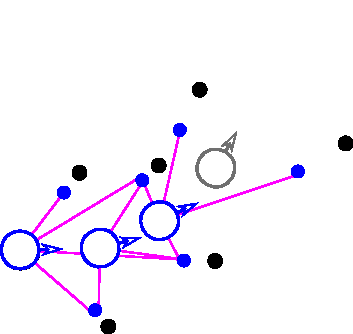
\includegraphics[width=0.44\textwidth]{slam_example_robot7.pdf}}
     }
     \end{figure}
    
    \end{frame}
    
    \begin{frame}
     \frametitle{SLAM example}
    
     \begin{figure}
     \subfloat[Reality]
     {
     \fbox{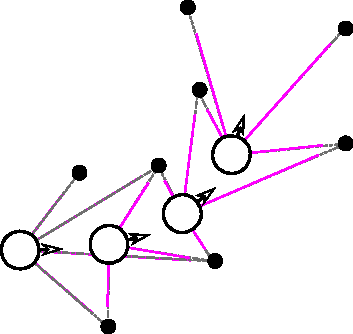
\includegraphics[width=0.44\textwidth]{slam_example_gt8.pdf}}
     }\hfill{}
     \subfloat[Robot SLAM system]
     {
     \fbox{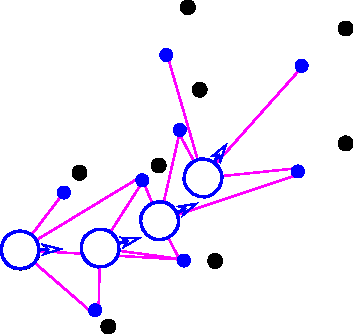
\includegraphics[width=0.44\textwidth]{slam_example_robot8.pdf}}
     }
     \end{figure}
    
    \end{frame}
    
    \begin{frame}
     \frametitle{General SLAM architecture}
    
     \begin{figure}[!h]
     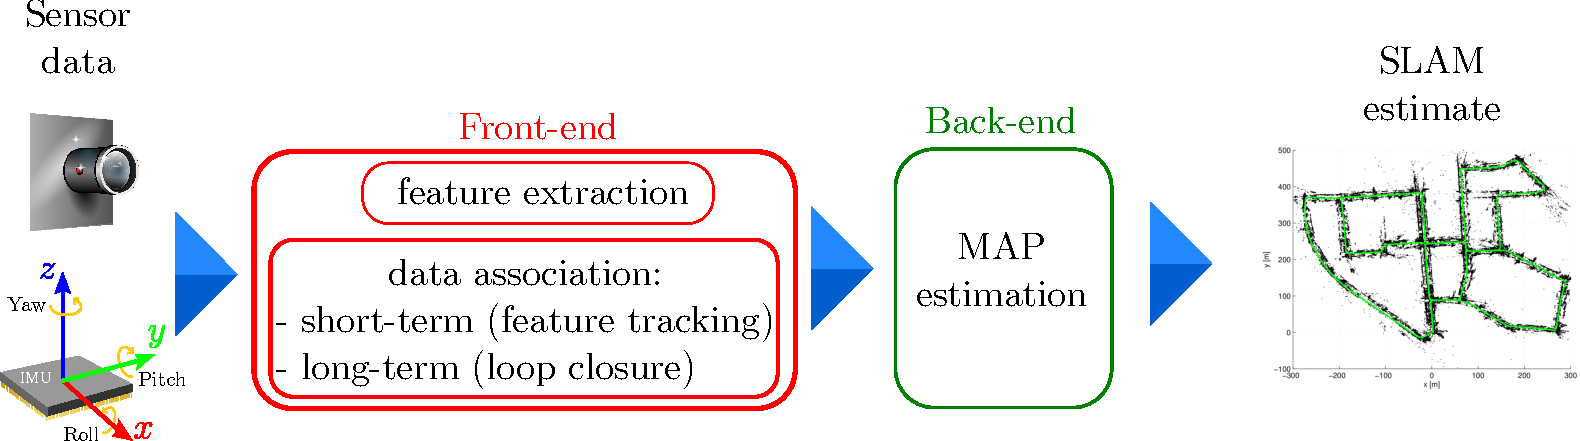
\includegraphics[width=\textwidth]{images/slam_frontend_backend.pdf}
     \end{figure}
    
\end{frame}

\begin{frame}
    \frametitle{Types of SLAM Back-ends}
    \note{Information taken from https://youtu.be/BuRCJ2fegcc and https://youtu.be/Alu59K8zvYs}
    \footnotesize
    \begin{itemize}
    \item Based on Kalman Filter (EKF-SLAM)
    \item Based on Particle Filter (FastSLAM, Rao-Blackwellized Particle Filter, Gmapping)
    \item Based on Least-Squares (Graph-SLAM, Bundle Adjustment)
    \begin{itemize}
    \item Pose-Graph (only contains the robot poses; the map is marginalized.\footnote{Marginalization is the process of removing variables without losing information.})
    \item Factor-Graph (contains poses and landmarks)
    \end{itemize}
    Optimization Tools
    \begin{itemize}
    \item Ceres
    \item GTSAM
    \item g2o
    \end{itemize}
    \end{itemize}
    
    \begin{center}
    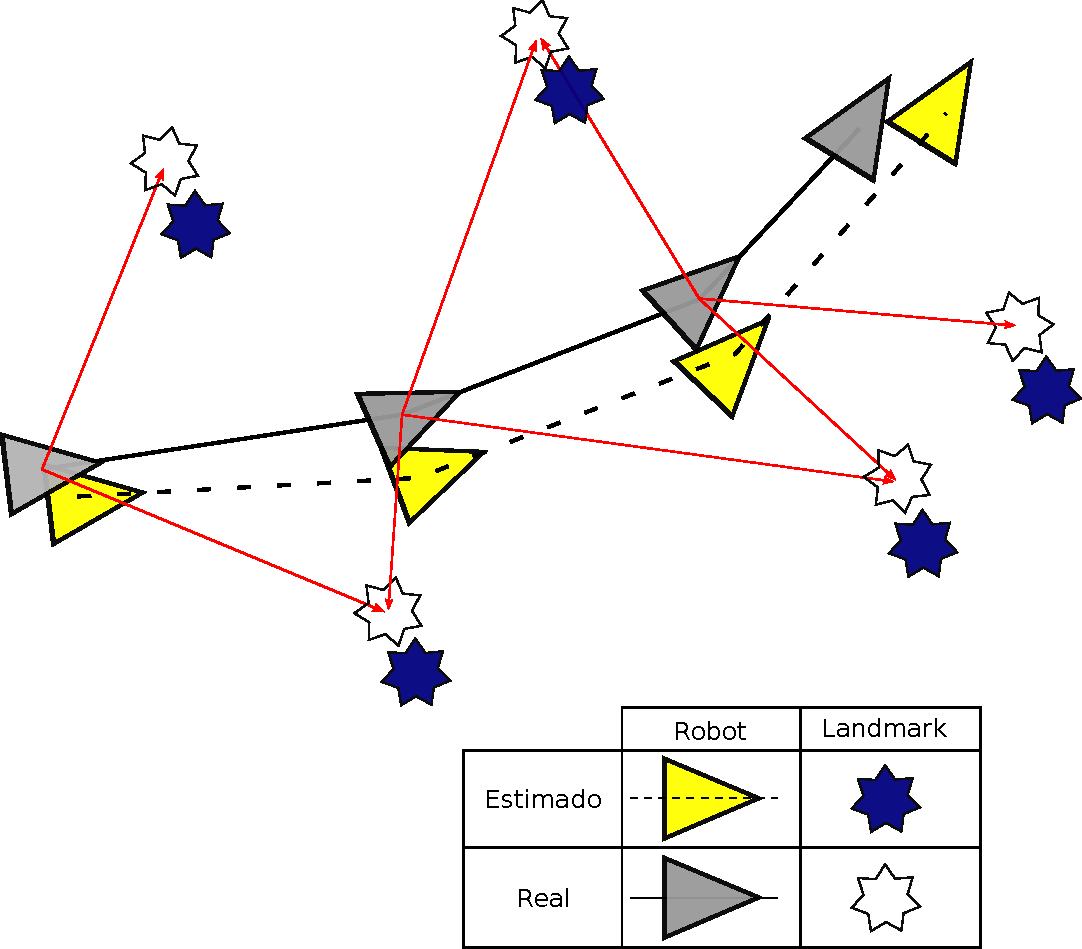
\includegraphics[width=0.25\textwidth]{images/slam-landmarks.pdf}
    \end{center}
    
    \end{frame}
    
    
    
    \section{Bundle Adjustment}
    \begin{frame}
    \frametitle{Material para Bundle Adjustment}
    \note{Extraído de Curso de Cyrill Stachniss https://youtu.be/LKDLcKrWOIU?si=InRBlf5Nmf7mGM9H}
    
    \TODO{Hacer slides de Bundle Adjustment}
    
    \begin{itemize}
        \item Cyrill Stachniss - The Basics about Bundle Adjustment
        
        Vídeo: \url{https://youtu.be/sobyKHwgB0Y?si=EqmuOjWNwKBI9jqH}
        
        Slides: \url{https://www.ipb.uni-bonn.de/html/teaching/photo12-2021/2021-pho2-09-BA-part1.pptx.pdf}
        \item Cyrill Stachniss - The Numerics of Bundle Adjustment
        
        Vídeo: \url{https://youtu.be/LKDLcKrWOIU?si=InRBlf5Nmf7mGM9H}
        
        Slides: \url{https://www.ipb.uni-bonn.de/html/teaching/photo12-2021/2021-pho2-10-BA-part2.pptx.pdf}
    \end{itemize}
\end{frame}

\begin{frame}
    \frametitle{Bundle Adjustment}
    \note{Información extraída de https://youtu.be/BuRCJ2fegcc y de https://youtu.be/mZBdPgBtrCM}
    
    Bundle Adjustment es un caso
    
    \begin{itemize}
        \item Reconstrucción 3D basada en imágenes tomadas de diferentes puntos de vista
        \item Minimiza el error de reproyección en el plano de la imagen 2D
        \item No hay noción de odometría (pose-pose constraints)
        \item En general utiliza como método de minimización Levenberg-Marquart
        \item Desarrollado en el área de Fotogrametría\footnote{Fotogrametría es la técnica cuyo objeto es estudiar y definir con precisión la forma, dimensiones y posición en el espacio de un objeto cualquiera, utilizando esencialmente medidas hechas sobre una o varias fotografías de ese objeto} durante la década de 1950
    \end{itemize}
    
\end{frame}

\begin{frame}
    \frametitle{Bundle Adjustment}
    
    \begin{figure}
        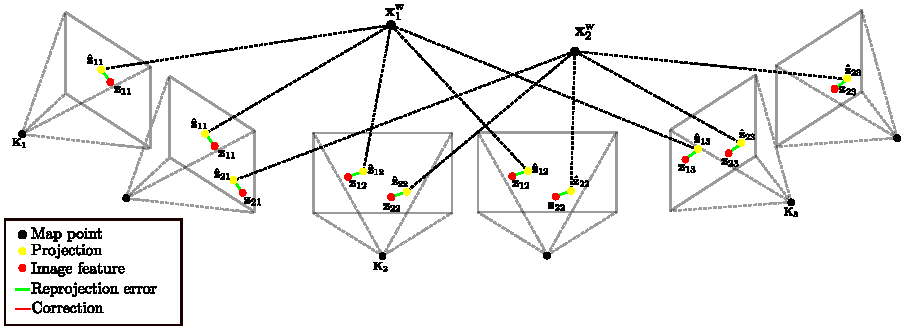
\includegraphics[width=\textwidth]{./images/ba_reprojection_error_before.pdf}
    \end{figure}
    
    \note{Ejemplo de ajuste de 3 keyframes que ven 2 puntos del mapa.\\
        k1 - x1 medición estéreo\\
        k1 - x2 medición derecha\\
        k2 - x1 medición estéreo\\
        k2 - x2 medición estéreo\\
        k3 - x1 medición izquierda\\
        k3 - x2 medición estéreo}
    
\end{frame}

\begin{frame}
    \frametitle{Bundle Adjustment}
    
    \begin{figure}
        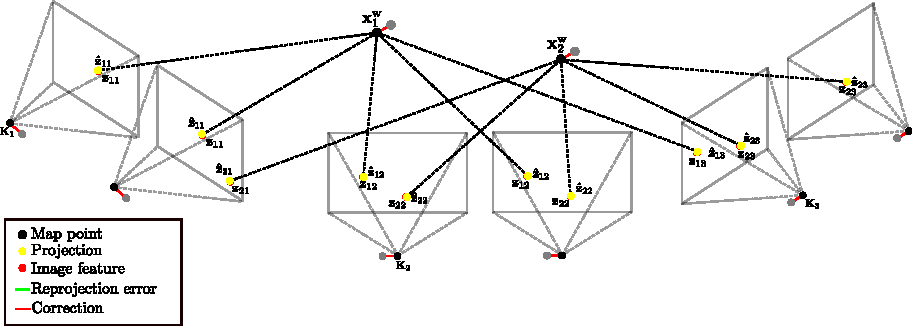
\includegraphics[width=\textwidth]{./images/ba_reprojection_error_after.pdf}
    \end{figure}
    
    \note{Ajustamos los keyframes y los puntos!!!\\
        Una ecuación de error por cada medición (6 en total).\\
        Nuevamente tenemos en cuenta la transformación rígida entre la cámara izquierda y la cámara derecha para las mediciones derechas.}
    
\end{frame}


\begin{frame}
    \frametitle{Bundle Adjustment}
    \note{Extraído de Cyrill Stachniss https://youtu.be/LKDLcKrWOIU?si=InRBlf5Nmf7mGM9H}
    
    Enfoque de mínimos cuadrados para estimar poses de cámara y puntos 3D
    
    \textbf{Idea Clave:}
    \begin{itemize}
        \item Comenzar con una solución inicial (\emph{initial guess})
        \item Proyectar los puntos 3D estimados en las imágenes de las cámaras estimadas
        \item Comparar ubicaciones de las proyecciones de los puntos 3D con los puntos medidos 2D
        \item Ajustar para minimizar el error en las imágenes
    \end{itemize}
    
\end{frame}

\begin{frame}
    \frametitle{Bundle Adjustment}
    \note{Extraído de Cyrill Stachniss https://youtu.be/LKDLcKrWOIU?si=InRBlf5Nmf7mGM9H}
    
    \TODO{Agregar contenido de Bundle Adjustment siguiendo el curso de Cyrill Stachniss}
    
\end{frame}



	
	\section{Bibliografía}
	\begin{frame}
	\frametitle{Bibliography}
   
    Static state binary Bayes filter:
    
    Capítulo 4.2 de \cite{thrun2005probabilistic}
    
    Occupancy Grid Mapping:
    
    Capítulo 9.1 y 9.2 de \cite{thrun2005probabilistic}
	
	\printbibliography
	
\end{frame}
	
\end{document}